\section{Theory} \label{sec:theory}

\subsection{The Helium atom}

\subsubsection{Ground state}
\begin{figure} [H]
	\begin{center}
		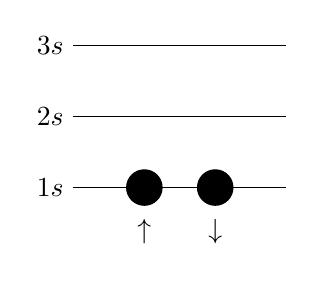
\begin{tikzpicture}[scale=0.9]
		\begin{scope}
			\foreach \i in {1,...,3}
			{
				\draw (-1,\i-1) node[anchor=east] {$\i s$} --(2,\i-1);
			}
			\filldraw (0,0) node[anchor=north,inner sep=.4cm] {$\uparrow$} circle (0.25cm); 
			\filldraw (1,0) node[anchor=north,inner sep=.4cm] {$\downarrow$} circle (0.25cm);
		\end{scope}
		\end{tikzpicture}
	\end{center}
\end{figure}

\subsubsection{Excited states}
\begin{figure} [H]
	\begin{center}
		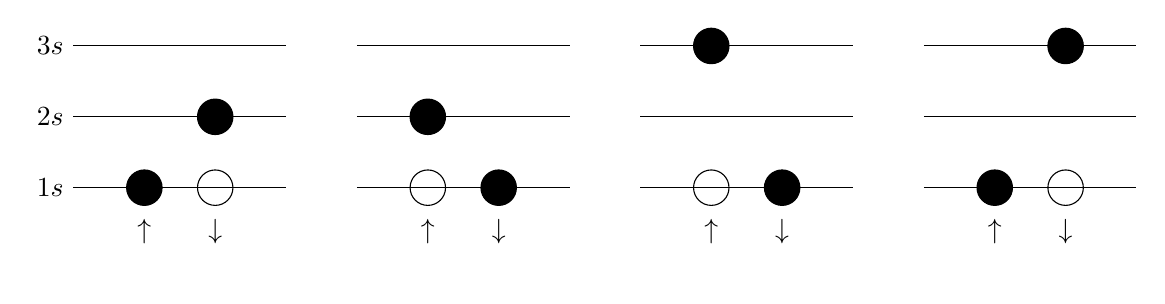
\begin{tikzpicture}[scale=0.9]
		\begin{scope}
		\foreach \i in {1,...,3}
		{
			\draw (-1,\i-1) node[anchor=east] {$\i s$} --(2,\i-1);
		}
		\filldraw (0,0) node[anchor=north,inner sep=.4cm] {$\uparrow$} circle (0.25cm); 
		\draw (1,0) node[anchor=north,inner sep=.4cm] {$\downarrow$} circle (0.25cm);
		\filldraw (1,1) circle (0.25cm);
		\end{scope}
		\begin{scope}[xshift=4cm]
		\foreach \i in {1,...,3}
		{
			\draw (-1,\i-1) --(2,\i-1);
		}
		\draw (0,0) node[anchor=north,inner sep=.4cm] {$\uparrow$} circle (0.25cm); 
		\filldraw (1,0) node[anchor=north,inner sep=.4cm] {$\downarrow$} circle (0.25cm);
		\filldraw (0,1) circle (0.25cm); 
		\end{scope}
		\begin{scope}[xshift=8cm]
		\foreach \i in {1,...,3}
		{
			\draw (-1,\i-1) --(2,\i-1);
		}
		\draw (0,0) node[anchor=north,inner sep=.4cm] {$\uparrow$} circle (0.25cm); 
		\filldraw (1,0) node[anchor=north,inner sep=.4cm] {$\downarrow$} circle (0.25cm);
		\filldraw (0,2) circle (0.25cm); 
		\end{scope}
		\begin{scope}[xshift=12cm]
		\foreach \i in {1,...,3}
		{
			\draw (-1,\i-1) --(2,\i-1);
		}
		\filldraw (0,0) node[anchor=north,inner sep=.4cm] {$\uparrow$} circle (0.25cm); 
		\draw (1,0) node[anchor=north,inner sep=.4cm] {$\downarrow$} circle (0.25cm);
		\filldraw (1,2) circle (0.25cm); 
		\end{scope}
		\end{tikzpicture}
		\newline
		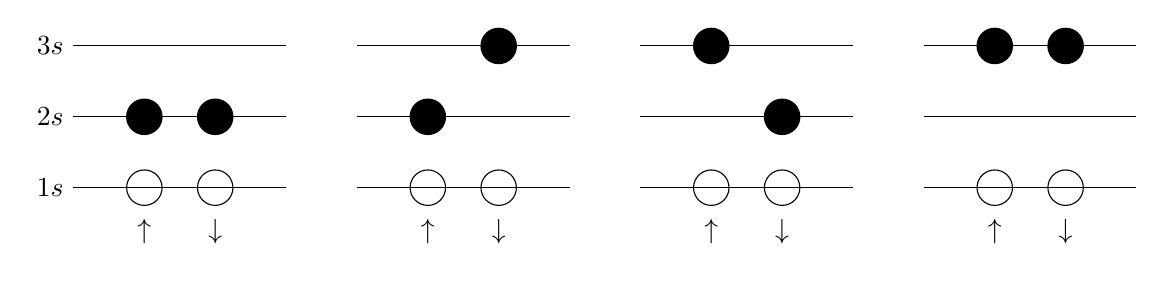
\begin{tikzpicture}[scale=0.9]
		\begin{scope}
		\foreach \i in {1,...,3}
		{
			\draw (-1,\i-1) node[anchor=east] {$\i s$} --(2,\i-1);
		}
		\draw (0,0) node[anchor=north,inner sep=.4cm] {$\uparrow$} circle (0.25cm); 
		\draw (1,0) node[anchor=north,inner sep=.4cm] {$\downarrow$} circle (0.25cm);
		\filldraw (0,1) circle (0.25cm);
		\filldraw (1,1) circle (0.25cm);
		\end{scope}
		\begin{scope}[xshift=4cm]
		\foreach \i in {1,...,3}
		{
			\draw (-1,\i-1) --(2,\i-1);
		}
		\draw (0,0) node[anchor=north,inner sep=.4cm] {$\uparrow$} circle (0.25cm); 
		\draw (1,0) node[anchor=north,inner sep=.4cm] {$\downarrow$} circle (0.25cm);
		\filldraw (1,2) circle (0.25cm);
		\filldraw (0,1) circle (0.25cm);
		\end{scope}
		\begin{scope}[xshift=8cm]
		\foreach \i in {1,...,3}
		{
			\draw (-1,\i-1) --(2,\i-1);
		}
		\draw (0,0) node[anchor=north,inner sep=.4cm] {$\uparrow$} circle (0.25cm); 
		\draw (1,0) node[anchor=north,inner sep=.4cm] {$\downarrow$} circle (0.25cm);
		\filldraw (0,2) circle (0.25cm); 
		\filldraw (1,1) circle (0.25cm); 
		\end{scope}
		\begin{scope}[xshift=12cm]
		\foreach \i in {1,...,3}
		{
			\draw (-1,\i-1) --(2,\i-1);
		}
		\draw (0,0) node[anchor=north,inner sep=.4cm] {$\uparrow$} circle (0.25cm); 
		\draw (1,0) node[anchor=north,inner sep=.4cm] {$\downarrow$} circle (0.25cm);
		\filldraw (0,2) circle (0.25cm); 
		\filldraw (1,2) circle (0.25cm);
		\end{scope}
		\end{tikzpicture}
	\end{center}
	\caption{\label{fig:schematic}}
\end{figure}

\subsection{The Beryllium atom}
\begin{figure}
	\begin{center}
		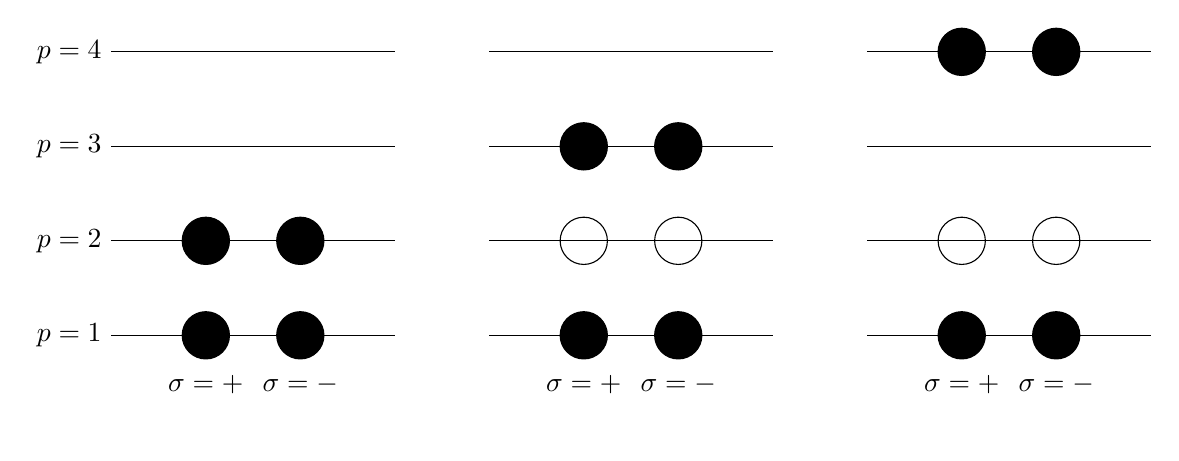
\begin{tikzpicture}[scale=1.2]
		\begin{scope}
		\foreach \i in {1,...,4}
		{
			\draw (-1,\i-1) node[anchor=east] {$p = \i$} --(2,\i-1);
		}
		\filldraw (0,0) node[anchor=north,inner sep=.5cm] {$\sigma=+$} circle (0.25cm); 
		\filldraw (1,0) node[anchor=north,inner sep=.5cm] {$\sigma=-$} circle (0.25cm);
		\filldraw (0,1) circle (0.25cm); 
		\filldraw (1,1) circle (0.25cm);
		\end{scope}
		\begin{scope}[xshift=4cm]
		\foreach \i in {1,...,4}
		{
			\draw (-1,\i-1) --(2,\i-1);
		}
		\filldraw (0,0) node[anchor=north,inner sep=.5cm] {$\sigma=+$} circle (0.25cm); 
		\filldraw (1,0) node[anchor=north,inner sep=.5cm] {$\sigma=-$} circle (0.25cm);
		\draw (0,1) circle (0.25cm); 
		\draw (1,1) circle (0.25cm);
		\filldraw (0,2) circle (0.25cm); 
		\filldraw (1,2) circle (0.25cm);
		\end{scope}
		\begin{scope}[xshift=8cm]
		\foreach \i in {1,...,4}
		{
			\draw (-1,\i-1) --(2,\i-1);
		}
		\filldraw (0,0) node[anchor=north,inner sep=.5cm] {$\sigma=+$} circle (0.25cm); 
		\filldraw (1,0) node[anchor=north,inner sep=.5cm] {$\sigma=-$} circle (0.25cm);
		\draw (0,1) circle (0.25cm); 
		\draw (1,1) circle (0.25cm);
		\filldraw (0,3) circle (0.25cm); 
		\filldraw (1,3) circle (0.25cm);
		\end{scope}
		\end{tikzpicture}
		\newline
		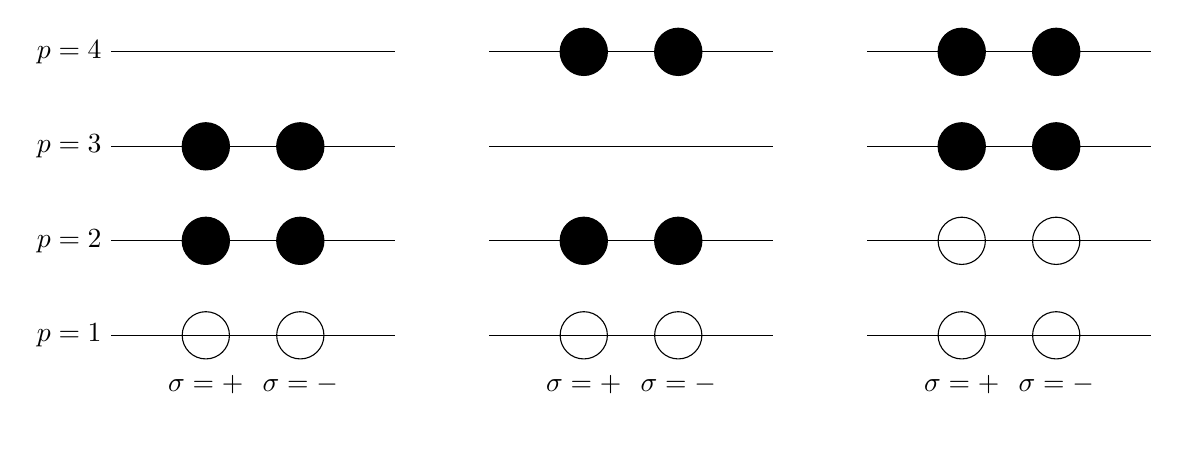
\begin{tikzpicture}[scale=1.2]
		\begin{scope}
		\foreach \i in {1,...,4}
		{
			\draw (-1,\i-1) node[anchor=east] {$p = \i$} --(2,\i-1);
		}
		\draw (0,0) node[anchor=north,inner sep=.5cm] {$\sigma=+$} circle (0.25cm); 
		\draw (1,0) node[anchor=north,inner sep=.5cm] {$\sigma=-$} circle (0.25cm);
		\filldraw (0,1) circle (0.25cm); 
		\filldraw (1,1) circle (0.25cm);
		\filldraw (0,2) circle (0.25cm); 
		\filldraw (1,2) circle (0.25cm);
		\end{scope}
		\begin{scope}[xshift=4cm]
		\foreach \i in {1,...,4}
		{
			\draw (-1,\i-1) --(2,\i-1);
		}
		\draw (0,0) node[anchor=north,inner sep=.5cm] {$\sigma=+$} circle (0.25cm); 
		\draw (1,0) node[anchor=north,inner sep=.5cm] {$\sigma=-$} circle (0.25cm);
		\filldraw (0,1) circle (0.25cm); 
		\filldraw (1,1) circle (0.25cm);
		\filldraw (0,3) circle (0.25cm); 
		\filldraw (1,3) circle (0.25cm);
		\end{scope}
		\begin{scope}[xshift=8cm]
		\foreach \i in {1,...,4}
		{
			\draw (-1,\i-1) --(2,\i-1);
		}
		\draw (0,0) node[anchor=north,inner sep=.5cm] {$\sigma=+$} circle (0.25cm); 
		\draw (1,0) node[anchor=north,inner sep=.5cm] {$\sigma=-$} circle (0.25cm);
		\draw (0,1) circle (0.25cm); 
		\draw (1,1) circle (0.25cm);
		\filldraw (0,2) circle (0.25cm); 
		\filldraw (1,2) circle (0.25cm);
		\filldraw (0,3) circle (0.25cm); 
		\filldraw (1,3) circle (0.25cm);
		\end{scope}
		\end{tikzpicture}
	\end{center}
	\caption{Above all basis states of our pair interaction system are presented schematically with $P=2$ as the number of pairs and $S_z=0$ are the total spin. The solid dots indicate occupied states, while the empty dots indicate unoccupied states (holes). The reference state $|\Phi\rangle$ is represented in the upper left corner. This is all possible states since the excusion principle does not allow two particles with same spin to stay at the same level. For further description, see the text.\label{fig:schematic}}
\end{figure}